% SPDX-License-Identifier: LPPL-1.3c
% Copyright (C) 2026 Christophe Jorssen
% Author and Current Maintainer: Christophe Jorssen <christophe.jorssen@gmail.com>
% LPPL maintenance status: maintained
% This file is part of luafemm. See LICENSE and LICENSES.md for its terms.
\section{A tutorial: finite electrodes and dielectric interfaces}
\label{sec:tutorial-electric-fe}

Kamil now wants to leave the ideal parallel-plate model. How does the field
bend around the end of a plate? What happens when only part of the gap contains
a dielectric? The analytical symmetry models cannot answer these questions.
He selects |model=finite elements| and describes the physical objects with
ordinary TikZ paths.

This is a \emph{planar} calculation: the section is extruded indefinitely
perpendicular to the page. A plate segment represents an infinite strip, not
a finite rectangular plate in three dimensions. A circular charged region
represents an infinite cylinder, not a sphere. The material law is
$\mathbf D=\epsilon_0\epsilon_r\mathbf E$, with positive scalar permittivity.

\luafemmexamplebegin{electric-fe-plates}
\subsection{Declare the electrodes before requesting a field}
Kamil gives the two electrodes names and signed potentials. A native TikZ pic
holds these declarations so that he can reuse the same geometry in several
independent calculations. A style collects the domain and mesh settings.
He invokes this physical pic with TikZ's |transform shape| option so that it
follows the picture's scale and rotation. Without it, native pics reset the
nontranslational transform; the electrodes would then change size relative to
the model's coordinate frame. Field-view pics already draw in that frame.

\begin{codeexample}[setup code]
\usetikzlibrary{backgrounds}
\tikzset{
  lesson electric box/.style={femm/electrostatic={model=finite elements,
    xmin=-3,xmax=3,ymin=-2,ymax=2,mesh size=.3}},
  lesson electric plates/.pic={
    \draw[very thick,femm/electric electrode={name=positive,potential=50}]
      (-.5,-1)--(-.5,1);
    \draw[very thick,femm/electric electrode={name=negative,potential=-50}]
      (.5,-1)--(.5,1);}}
\end{codeexample}

The physical coordinate unit is still one centimetre. Here, however, |xmin|,
|xmax|, |ymin| and |ymax| define a \emph{computational domain}, not just a crop.
By default its exterior is held at zero potential. That is a finite grounded
boundary, and its distance from the plates will need checking.

\begin{codeexample}[width=0pt]
\begin{tikzpicture}[lesson electric box,
    femm/electrostatic={name=fe coarse},scale=.8]
  \pic[transform shape] {lesson electric plates};
  \begin{scope}[on background layer]
    \pic {femm electric mesh};
    \pic[femm/electric={lines per charge=20}] {femm electric field};
  \end{scope}
  \draw[gray,densely dotted] (-3,-2) rectangle (3,2);
  \node[above] at (-.5,1) {$+50\,\mathrm V$};
  \node[below] at (.5,-1) {$-50\,\mathrm V$};
  \path[femm/electric profile={name=fe coarse axis,samples=101}]
    (0,-1.8)--(0,1.8);
\end{tikzpicture}
\end{codeexample}

The mesh conforms to the electrode paths. The first mesh request fixes the
physical declarations; the first field or profile request also solves the
linear system. There is no magnetic |\femmsolve| call. Kamil must declare
\emph{every} dielectric, source, electrode and boundary before either request.
Drawing ordinary labels afterwards is harmless; adding another physical path
is rejected. Saving a named model at the end of the picture also requests a
solution, so it can be reused with its owned mesh and potential.

The field near a plate end is no longer uniform. For an ideally sharp,
zero-thickness edge its pointwise magnitude is singular in the continuum
model. Kamil should not interpret the largest raw triangle value as a converged
physical maximum. He measures on the symmetry axis between the plates,
away from their endpoints.

\subsection{Refine the mesh, then move the exterior boundary}
A coarse mesh makes initial layout and declaration checks quick. Once those
are correct, Kamil reduces |mesh size| by a factor of two. Equipotentials now
come directly from the piecewise linear solved potential; increasing the
analytical renderer's |contour resolution| would not improve this FE solution.

\begin{codeexample}[width=0pt]
\begin{tikzpicture}[lesson electric box,
    femm/electrostatic={mesh size=.15,name=fe fine},scale=.8]
  \pic[transform shape] {lesson electric plates};
  \begin{scope}[on background layer]
    \pic[femm/electric={lines per charge=24}] {femm electric field};
    \pic[femm/electric={levels={-40,-20,0,20,40}}] {femm equipotentials};
  \end{scope}
  \draw[gray,densely dotted] (-3,-2) rectangle (3,2);
  \path[femm/electric profile={name=fe fine axis,samples=161}]
    (0,-1.8)--(0,1.8);
\end{tikzpicture}
\end{codeexample}

Mesh refinement alone converges to the finite-box problem. Kamil therefore
performs a separate experiment: he keeps the finer mesh size and moves the
zero-potential boundary farther away. The drawing below shows only a central
window. The |femm/electric| view keys crop the field without moving the
physical boundary at five centimetres. He seeds the lines along the central
axis so that every requested line starts inside this crop. Automatic seeds on
remote voltage edges would otherwise be hidden by the restricted view.
The dotted rectangle below marks this view window, not a physical boundary.

\begin{codeexample}[width=0pt]
\begin{tikzpicture}[lesson electric box,femm/electrostatic={
    xmin=-5,xmax=5,ymin=-5,ymax=5,mesh size=.15,name=fe wide}]
  \pic[transform shape] {lesson electric plates};
  \path[femm/electric seeds={samples=17}] (0,-1.8)--(0,1.8);
  \pic[femm/electric={xmin=-2,xmax=2,ymin=-2,ymax=2}]
    {femm electric field};
  \draw[gray,densely dotted] (-2,-2) rectangle (2,2);
  \path[femm/electric profile={name=fe wide axis,samples=161}]
    (0,-1.8)--(0,1.8);
\end{tikzpicture}
\end{codeexample}

The graph compares $E_x$ along the $y$ axis. The gaps between short horizontal
pieces are deliberate: the first-order FE field is constant in each triangle,
and no recovered or smoothed field has been substituted. The potential itself
is continuous. Refining |samples| only adds measurements to the existing
solution; it cannot replace refining the physical mesh.

\begin{codeexample}[width=0pt]
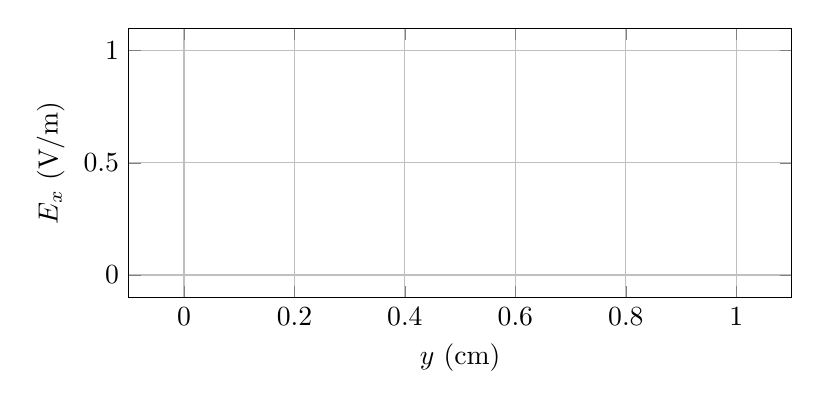
\begin{tikzpicture}
\begin{axis}[width=10cm,height=5cm,no markers,grid=major,
  xlabel={$y$ (cm)},ylabel={$E_x$ (V/m)},
  legend style={at={(.5,1.03)},anchor=south,legend columns=3}]
  \femmelectricplot[profile=fe coarse axis,component=Ex,abscissa=y,
    plot options={gray,thick}]
  \addlegendentry{Coarse}
  \femmelectricplot[profile=fe fine axis,component=Ex,abscissa=y,
    plot options={blue!70!black,thick}]
  \addlegendentry{Fine}
  \femmelectricplot[profile=fe wide axis,component=Ex,abscissa=y,
    plot options={red!70!black,thick}]
  \addlegendentry{Wider box}
\end{axis}
\end{tikzpicture}
\end{codeexample}

Kamil can also compare the electrode charge per extrusion length. The named
electrode's charge is obtained from the discrete variational reaction, not
from an arbitrary contour through the discontinuous raw field. The artificial
exterior boundary participates in charge balance and must not be forgotten.

\begin{codeexample}[width=0pt]
\begin{tabular}{lr}
Calculation & Positive electrode charge per length (C/m)\\
Coarse & \femmelectricvalue[model=fe coarse,electrode=positive,
  quantity=charge per length]\\
Fine & \femmelectricvalue[model=fe fine,electrode=positive,
  quantity=charge per length]\\
Wider box & \femmelectricvalue[model=fe wide,electrode=positive,
  quantity=charge per length]
\end{tabular}
\end{codeexample}

The changes between these calculations are sensitivity evidence, not a
universal error estimate. A final course figure should state its planar
interpretation and show the physical assumptions that matter.
\luafemmexampleend{electric-fe-plates}

\luafemmexamplebegin{electric-fe-dielectrics}
\subsection{Put a dielectric in half of the gap}
For a controlled comparison Kamil first removes the edge effects. The top and
bottom of a rectangular domain are insulating, meaning $\mathbf D\cdot\mathbf n=0$.
Its left and right sides are electrodes. A closed TikZ region changes the
relative permittivity in the left half from one to four. This geometry has an
exact piecewise linear potential, so linear triangles can reproduce it to the
linear solver tolerance.

\begin{codeexample}[width=0pt]
\begin{tikzpicture}[femm/electrostatic={model=finite elements,
    xmin=0,xmax=2,ymin=-.7,ymax=.7,outer boundary=insulated,
    mesh size=.15,name=fe dielectric},scale=1.4]
  \draw[fill=blue!10,draw=none,
    femm/electric region={relative permittivity=4}]
    (0,-.7) rectangle (1,.7);
  \draw[very thick,femm/electric electrode={name=left,potential=100}]
    (0,-.7)--(0,.7);
  \draw[very thick,femm/electric electrode={name=right,potential=0}]
    (2,-.7)--(2,.7);
  \pic[femm/electric={lines per charge=7}] {femm electric field};
  \pic[femm/electric={levels={20,40,60,80}}] {femm equipotentials};
  \node[above] at (.5,.7) {$\epsilon_r=4$};
  \node[above] at (1.5,.7) {$\epsilon_r=1$};
  \path[femm/electric profile={name=fe dielectric radius,samples=2}]
    (0,0)--(2,0);
\end{tikzpicture}
\end{codeexample}

The requested two uniform profile samples would miss the material interface.
The profile inserts every intersected mesh edge and retains both field limits.
Here $E_x$ jumps by a factor of four while $D_x$ stays constant. This is a
physical discontinuity, which must survive any choice of plotting samples.

\begin{codeexample}[width=0pt]
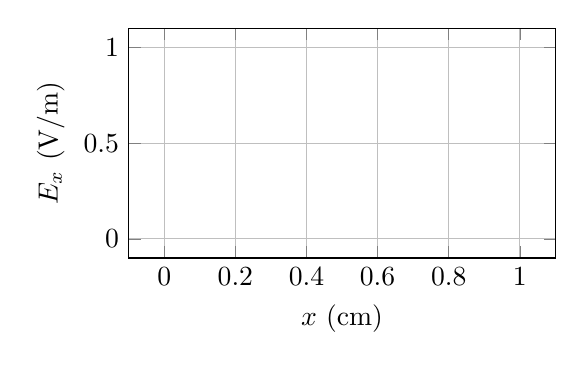
\begin{tikzpicture}
\begin{axis}[width=7cm,height=4.5cm,no markers,grid=major,
  xlabel={$x$ (cm)},ylabel={$E_x$ (V/m)}]
  \femmelectricplot[profile=fe dielectric radius,component=Ex,abscissa=x,
    plot options={blue!70!black,thick}]
\end{axis}
\end{tikzpicture}
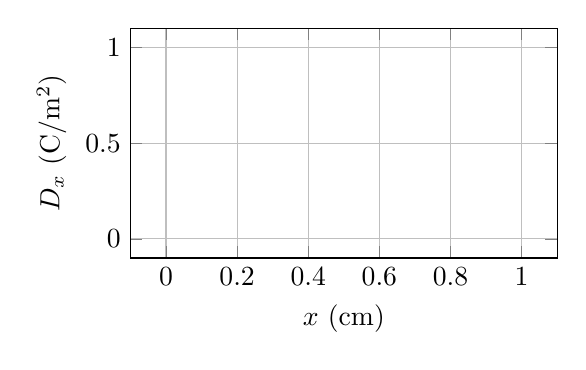
\begin{tikzpicture}
\begin{axis}[width=7cm,height=4.5cm,no markers,grid=major,
  xlabel={$x$ (cm)},ylabel={$D_x$ (C/m$^2$)}]
  \femmelectricplot[profile=fe dielectric radius,component=Dx,abscissa=x,
    plot options={red!70!black,thick}]
\end{axis}
\end{tikzpicture}
\end{codeexample}

At an arbitrary point exactly on a mesh face, the raw sampler chooses the
lowest-index incident element. Crossing profiles instead retain both limits.
No unique normal electric field should be inferred at a dielectric jump.
Ordinary TikZ transformations change the view; a locally transformed physical
path changes the material geometry before the solve.

\subsection{Replace the dielectric interface by a charged layer}
Kamil now uses vacuum everywhere, grounds both electrodes, and prescribes a
uniform positive surface charge at $x=1$ cm. In this planar interpretation the
line is an infinite sheet perpendicular to the section. Its input is a surface
density in $\mathrm{C/m^2}$, not the charge in coulombs of a point-charge node.

\begin{codeexample}[width=0pt]
\begin{tikzpicture}[femm/electrostatic={model=finite elements,
    xmin=0,xmax=2,ymin=-.7,ymax=.7,outer boundary=insulated,
    mesh size=.15,name=fe sheet},scale=1.4]
  \draw[very thick,femm/electric electrode={name=left,potential=0}]
    (0,-.7)--(0,.7);
  \draw[very thick,femm/electric electrode={name=right,potential=0}]
    (2,-.7)--(2,.7);
  \draw[red!70!black,thick,
    femm/electric charge layer={surface charge density=1e-9}]
    (1,-.7)--(1,.7);
  \pic[femm/electric={lines per charge=12}] {femm electric field};
  \pic[femm/electric={levels={.1,.2,.3,.4,.5}}] {femm equipotentials};
  \path[femm/electric profile={name=fe sheet radius,samples=21}]
    (0,0)--(2,0);
\end{tikzpicture}
\end{codeexample}

\begin{codeexample}[width=0pt]
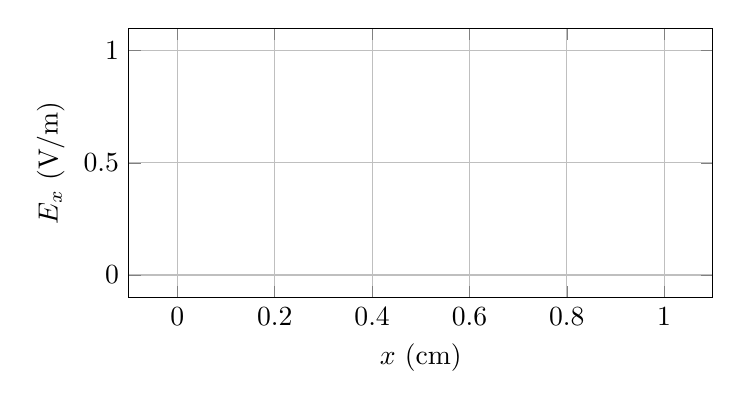
\begin{tikzpicture}
\begin{axis}[width=9cm,height=5cm,no markers,grid=major,
  xlabel={$x$ (cm)},ylabel={$E_x$ (V/m)}]
  \femmelectricplot[profile=fe sheet radius,component=Ex,abscissa=x,
    plot options={blue!70!black,thick}]
\end{axis}
\end{tikzpicture}
\end{codeexample}

The field points away from the sheet. Its displacement jump is $\sigma$,
and the potential is continuous. A charged layer is an internal dielectric
source; it cannot simultaneously be a voltage electrode. The two grounded
electrodes acquire compensating charges through their voltage constraints.
\luafemmexampleend{electric-fe-dielectrics}

\luafemmexamplebegin{electric-fe-charge}
\subsection{A charged cylinder inside a grounded tube}
For one final check, Kamil returns to an analytical case. The circular region
has radius one centimetre and uniform volume charge
$\rho=10^{-7}\,\mathrm{C/m^3}$. A grounded circular electrode at radius two
centimetres fixes the potential reference. It encloses dielectric material,
so Kamil must set |interior=dielectric|. A closed electrode otherwise represents
a solid conductor, with constant potential throughout its interior.

\begin{codeexample}[width=0pt]
\begin{tikzpicture}[femm/electrostatic={model=finite elements,
    xmin=-2.4,xmax=2.4,ymin=-2.4,ymax=2.4,mesh size=.15,
    name=fe charged cylinder}]
  \draw[fill=red!8,draw=red!60!black,
    femm/electric region={volume charge density=1e-7,
      mesh size=.1,curve tolerance=.0005}]
    (0,0) circle[radius=1];
  \draw[thick,femm/electric electrode={name=tube,potential=0,
      interior=dielectric,curve tolerance=.0005}]
    (0,0) circle[radius=2];
  \pic[femm/electric={lines per charge=20}] {femm electric field};
  \pic[femm/electric={levels={.1,.2,.3,.4,.5}}] {femm equipotentials};
  \path[femm/electric profile={name=fe cylinder radius,samples=101}]
    (0,0)--(1.9,0);
\end{tikzpicture}
\end{codeexample}

The original TikZ drawing remains a circle. The mesh uses flattened physical
segments controlled by |curve tolerance|. Both geometric approximation and
mesh spacing need refinement for a quantitative comparison. The analytical
provider supplies the reference graph without a second numerical mesh:

\begin{codeexample}[width=0pt]
\begin{tikzpicture}[femm/electrostatic={model=charged cylinder,radius=1,
    volume charge density=1e-7,reference radius=2}]
  \pic {femm electric geometry};
  \path[femm/electric profile={name=exact cylinder radius,samples=161}]
    (0,0)--(1.9,0);
\end{tikzpicture}
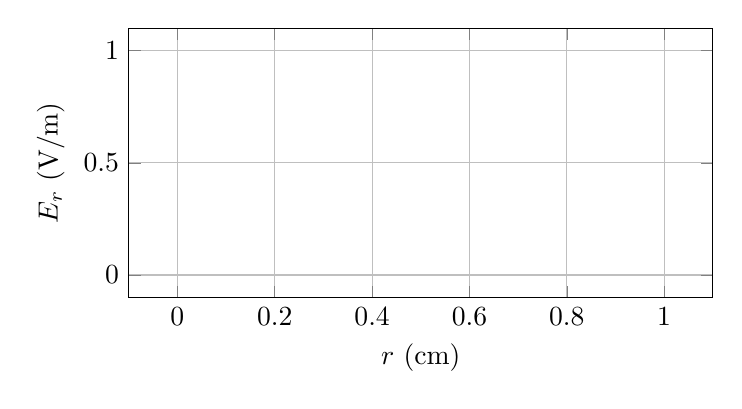
\begin{tikzpicture}
\begin{axis}[width=9cm,height=5cm,no markers,grid=major,
  xlabel={$r$ (cm)},ylabel={$E_r$ (V/m)},
  legend style={at={(.5,1.03)},anchor=south,legend columns=2}]
  \femmelectricplot[profile=exact cylinder radius,component=Ex,abscissa=x,
    plot options={black,dashed}]
  \addlegendentry{Analytical}
  \femmelectricplot[profile=fe cylinder radius,component=Ex,abscissa=x,
    plot options={blue!70!black,thick}]
  \addlegendentry{Finite elements}
\end{axis}
\end{tikzpicture}
\end{codeexample}

Kamil distinguishes three controls: |curve tolerance| approximates the physical
boundary, |mesh size| approximates the solution, and |samples| samples that
solution for a graph. The FE field near the centre need not be exactly zero
on a finite asymmetric mesh. A smooth-looking graph alone would not establish
accuracy; the comparison and refinement are what make the figure useful.
\luafemmexampleend{electric-fe-charge}
